\documentclass[twocolumn]{article}\usepackage[english]{babel}
\usepackage[utf8x]{inputenc}
\usepackage{pdfpages}
\usepackage{amsmath}
\usepackage{siunitx}
\usepackage{hyperref}
\usepackage{graphicx}
\usepackage[colorinlistoftodos]{todonotes}
\usepackage[]{mcode}
\usepackage{tikz}
\usepackage{circuitikz}
\usepackage{placeins}
\title{Using a Lock-In amplifier to determine filters from High Pass Circuits}
\author{Aaron Kebede}
\date{\today}
\begin{document}
\maketitle
\begin{abstract}

This report provides insight into the analysis of R-C circuits using signal generators. We study circuits in three steps. First, we study a very simple circuit just consisting of a resistor, a capacitor element, and a signal generator. The signal generator generates a current with a specific frequency which we can then vary to study the effects on the other circuit elements. Second, we create a virtual instrument(using LabVIEW) program to automate alteration of the frequency and third, we add a lock-in amplifier in the circuit to extract all the signals and automate our process of collecting the data. We find that for large frequencies, the phase shift is slightly negatively correlated with the frequency while the amplitude has a strong positive correlation. The data, its analysis, and full plots are available at \url{https://220.kebede.org}\footnote{The website contains documentation on how to use the code, how the data is arranged, the nomenclature of the saved data folder}

\end{abstract}

\section{Introduction}

Included in this report are details of the method, graphs, results, error analysis, discussions and conclusions of results. We record data and analyze it to find correlations between signals sent from the signal generator and the feedback from the circuit recorded in different sets.  
\newline

\section{Background}
\subsection{RC Circuits}
RC circuits, as the name indicates, are circuits that consist of resistance and capacitance elements. One may think that these circuits would not be of no specific interest, if speaking based solely on how individual resistor and capacitor circuits behave. However, when we have a capacitor and resistor in the same circuit, we start observing some interesting phenomena. One common interesting occurrence is the time constant denoted by the Greek letter, $\tau$(tau). $\tau$ is the product of the capacitance and resistance in the circuit.
\newline
\newline
\newline
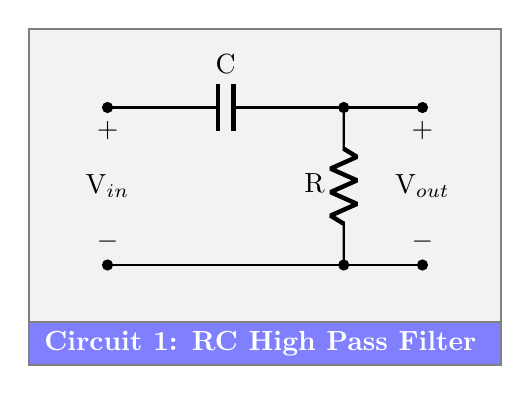
\begin{tikzpicture}[american,thick]
 
% Change components size
\ctikzset{
    resistors/scale=0.8,
    capacitors/scale=0.7,
}
% Orange boxes
\draw
[
    fill=black!5,
    draw=black!50
] (-1,-0.75) rectangle(5,3);
 
\node
[
    align=center,
    minimum width=6cm,
    fill=blue!50,
    text=white,
    draw=black!50
] at (2,-1){\textbf{Circuit 1: RC High Pass Filter} };
% Circuit code
\draw (0,0) to[short,*-*] ++ (4,0);
\draw (0,2) to[C=C,*-] ++ (3,0) coordinate(a);
\draw (a) to[short,-*] ++ (1,0);
\draw (a) to[R,l_=R,*-*] ++(0,-2);
% Voltage labels
\draw (0,2) to[open,v=V$_{in}$] ++(0,-2);
\draw (4,2) to[open,v=V$_{out}$] ++(0,-2);
\end{tikzpicture}
\newline
\newline
\newline

The time constant tells us important properties about how the circuit behaves. For instance, we can find out experimentally, how the time constant is related to the voltage drop in the circuit. Although we won't be performing an experiment to verify this(as this is a known fact) in our lab, we can use use some publicly available information to verify this. To do this, we performed a simulation on Circuit Lab\footnote{Circuit Lab is an online Circuit Simulation software}. On Circuit Lab, we created a circuit that emulated the properties and set up of the circuit we had in the lab. We then run the simulation, collected the data and visualized it only to discover that it behaves the same as theoretically predicted.
\newline
\newline
The theoretical prediction of a Voltage charging curve against time is that it will be an exponential curve that relates the voltage at each time with the source voltage. It can be mathematically proven as follows;
Let's apply Kirchhoff's Rule to our circuit in \textbf{Figure 2}.\newline

\(V_{in} - V_{R} - V_{C} =0\), \newline \newline Where V$_{R}$ and V$_{C}$ are voltages in the Resistor and Capacitor respectively. \newline \newline
V$_{C}$ - IR - $\frac{q}{C}$= 0, \newline \newline Where I is the current in the circuit and q is the charge in the capacitor.\newline \newline
V$_{in}$ - R$\frac{dq}{dt}$ - $\frac{q}{C}$ = 0, \newline \newline
$\frac{dq}{dt}$ = $\frac{V_{in}C-q}{RC}$, \newline \newline
\(\int_0^q \frac{dq}{V_{in}C-q} = \frac{1}{RC} \int_0^t dt\), \newline \newline
\text{Simplifying using integration by parts, we get} \newline \newline
\(\frac{V_{in}C - q}{V_{in}C} = e^{-t/RC}\), \newline \newline
\(q(t) = V_{in}C  \left(1 - e^{-\frac{t}{RC}}\right)\) \newline \newline
\(q(t)=Q\left(1 - e^{-\frac{t}{\tau}}\right)\) \newline \newline
\(V(t) = Cq(t)\) \newline \newline
\(V(t)=CQ\left(1 - e^{-\frac{t}{\tau}}\right)\) \newline \newline
\(V(t) = V_{in}\left(1 - e^{-\frac{t}{\tau}}\right)\) ... \textbf{equation 1} \newline \newline
Here, we discover a very important property when V is V($\tau$). This implies that \(V(\tau) = V_{in}\left(1 - \frac{1}{e}\right)\).
\newline \newline
Below are the two voltage curves we made from our simulation - one using a frequency generator and another one as a DC source for the voltage sources. We see in both cases, that the curves follow a general exponential curve. From our derivation above, we have seen that the voltage at any time can be found using equation 1. Our capacitance and resistance values for the circuit were 22nF and \SI{1.5}{M\ohm} respectively from which we can calculate the time constant. \newline
\begin{figure}
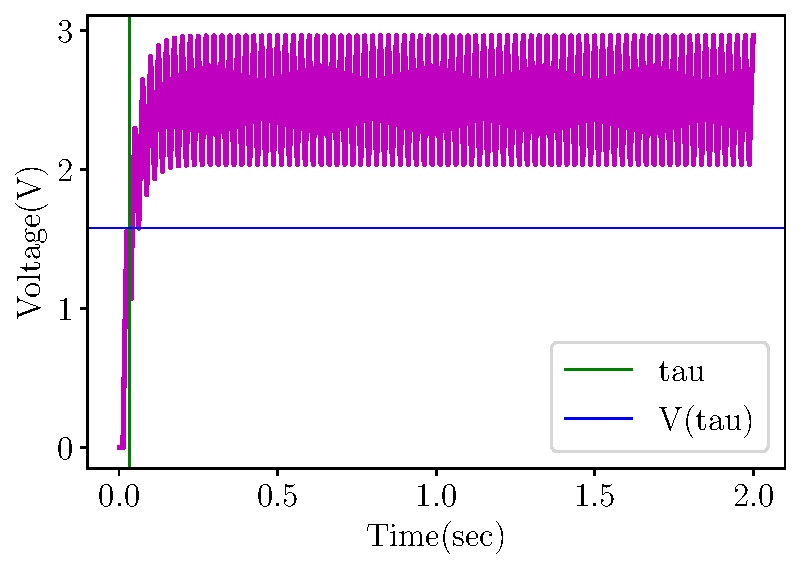
\includegraphics[width=\linewidth]{images/v2/Signal Generated RC Circuit Plot.pdf}
\caption{\textbf{V} vs \textbf{T} curve in a circuit where the source is signal generated }
  \label{fig:Signal RC Voltage}
\end{figure}

\begin{figure}
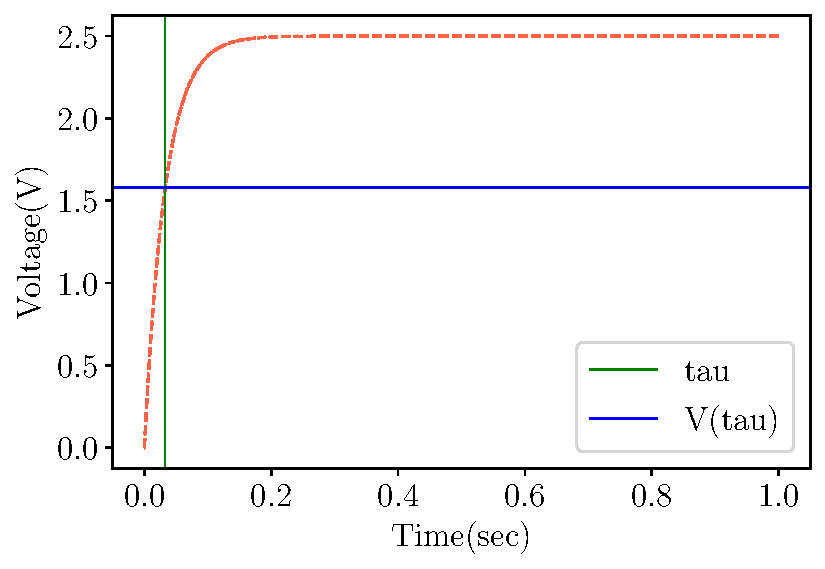
\includegraphics[width=\linewidth]{images/v2/RC Circuit Plot.pdf}
\caption{\textbf{V} vs \textbf{T} curve in a circuit where the source is DC voltage.  }
  \label{fig:DC RC Voltage}
\end{figure}

From the curve and experimental data, we can see that the initial voltage
$V_i$ after some time, t, drops to $V_t$. When it is at the time
constant(\textit{i.e.}), t=$\tau$, \newline \newline
\(V(\tau) = V_{in}\left(1 - e^{-\frac{\tau}{\tau}}\right)\) \newline
\(V(\tau) = V_{in}\left(1-\frac{1}{e}\right)\) \newline 

When plotting the experimental data, we labeled the the values of $\tau$ and V($\tau$) to see how the experiment would behave. We find that the experimental results indeed fully match the expected theoretical values as we have presented in Figures 2 and 3. The blue horizontal lines denote V($\tau$) while $\tau$ is represented as the green vertical line on both figures.   
\subsection{High Pass Circuits}
As the name indicates, a high pass filter is a type of circuit filter that lets high frequency signals pass while impeding low frequency(below a certain threshold) signals. Some real life applications of high pass filters include being used as audio filters, or in signal blocking for frequencies below a certain threshold. To construct a high pass filter, we created a circuit that resembles the one that we see at Circuit 1. Theoretically, the way a high pass filter works by leveraging the properties of a capacitor. When designing high pass filters, we connect the signal generator or source to the capacitor for two reasons. First, since its responses to different input signals are different and secondly, it takes time for a capacitor to charge and discharge as we have seen in the section above. 
When we connect the input directly to the capacitor and connect the capacitor in parallel to the resistor, the capacitor lets high frequencies pass while the current below a certain frequency becomes zero. This happens because the capacitor has high capacitance at low frequencies which blocks current flow in the circuit, but after a certain increase in the frequency, the capacitance decreases and hence current flow is possible.
\section{Methods}
\subsection{Set Up and Procedures}
\begin{figure}
  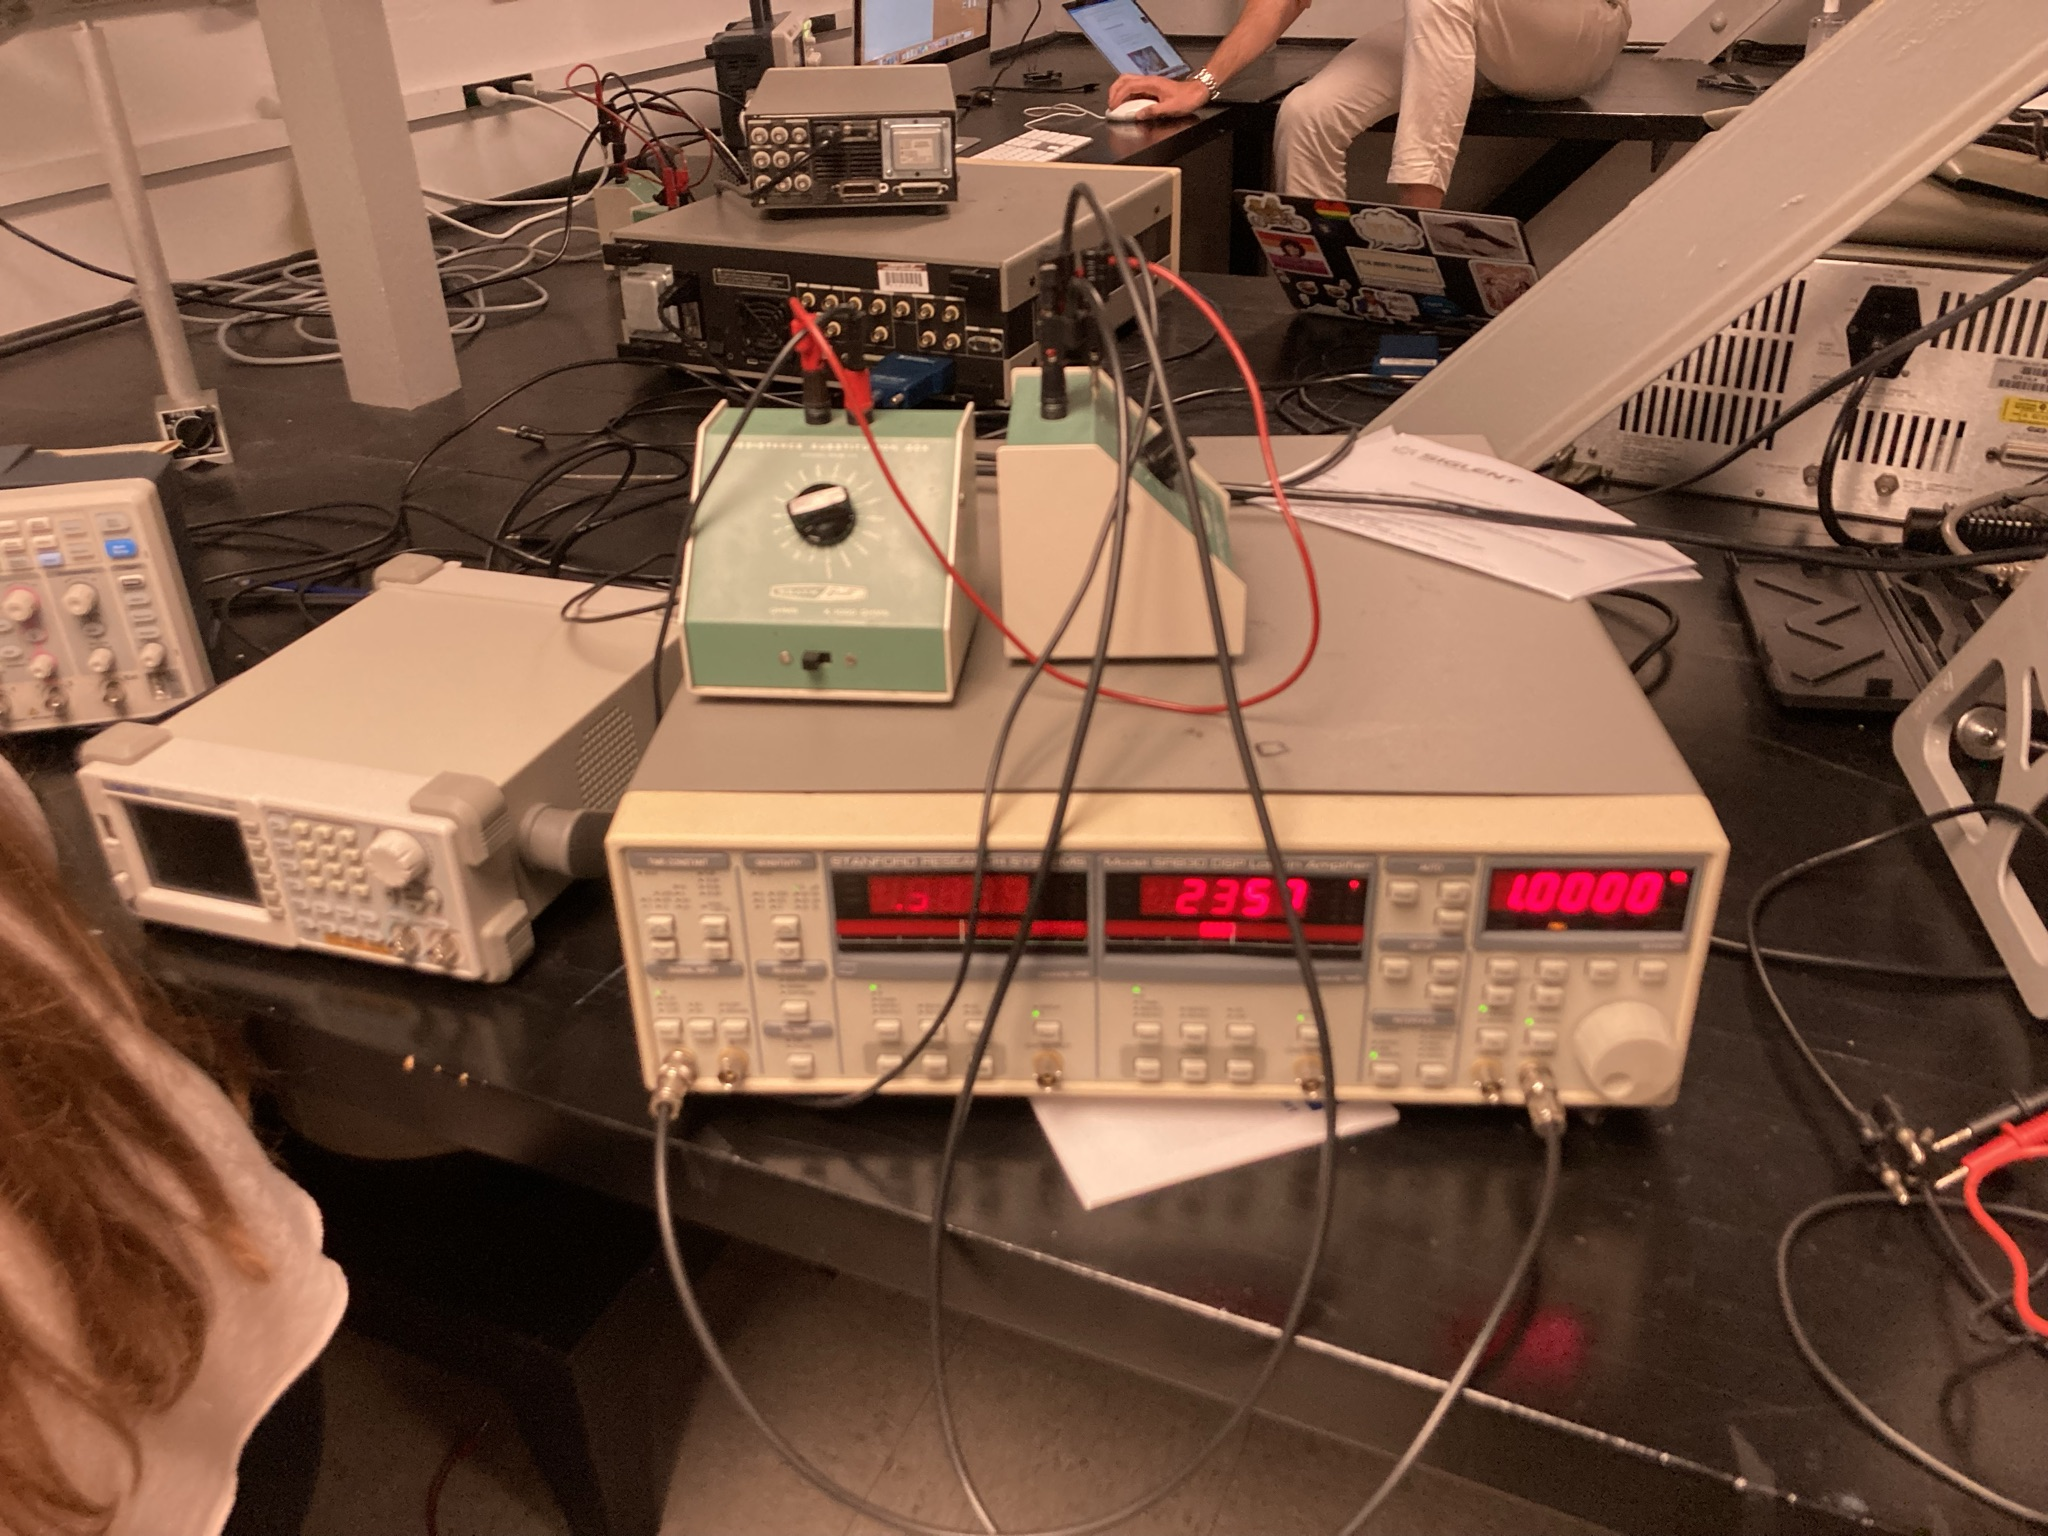
\includegraphics[width=\linewidth]{images/lab/setup.JPEG}
  \caption{Our lab setup}
  \label{fig:LAB_SETUP}
\end{figure}

We performed our data collection in three steps:
\newline
\begin{Steps}
 \item{\textbf{1.} We set up a circuit with a variable resistor, variable capacitor, and  a function generator. We varied the signal on the function generator and then recorded the data \textbf{by hand} on an excel sheet. Steps like this generally help get started on an experiment and guide on if we are on the right track.} 
 \item{\textbf{2.} We then created a LabVIEW program to automate the signals that were being generated. } 
 \item{\textbf{3.} Then, we added an amplifier to the circuit as shown in \textbf{Figure 3} above. We sent signals to the circuit using the LabVIEW program we created in Step 2. We record data automatically into an excel sheet and we start analyzing out output as will be discussed in the \textbf{Results} section.}
\end{Steps} \newline

\subsection{Data Structure}
\begin{tikzpicture}
\node {Root Directory} [sibling distance = 4cm, level distance = 3cm]
    child {node {Hand Recorded Data}} 
    child {node {v1}
    child {node {AMP}}
    child {node {FREQ}}
    child {node {PS}}}
    child {node {v2}
    child {node {LA}
    child {node {P vs F}}
    child {node {A vs F}}}
    child {node {DEF}
    child {node {A vs F}}
    child {node {P vs F}}}};
\end{tikzpicture}
Although we did not use some of the data that was collected, mostly because we were measuring the wrong things or the data sets were too small(as was the case in the hand recorded data), it was a good insight to have on whether we wanted to do the experiment the way it was or if we had to tweak some of the values from the signal generator, or change the capacitance and resistance so that the results we were trying to show would best be represented. As we have explained in the documentation code, organized the data into CSV/XLSX files. Although the default output of the recorded data from LabVIEW is in the excel format, we change the format to CSV in order to make it easier to use it with software libraries like numpy and pandas. We had three major recordings of the data that we categorized into three groups. One is the hand recorded data, the second one is v1, and the third one is v2. v2 is the most recent and main data of the experiment. v1 is the first version of the data that was collected using LabVIEW before incorporating the amplifier in the circuit. We added the amplifier and recollected data into v2. In the latest version, v2, The data is organized into 4 files. Two of the files are \textit{Amplitude vs Frequency} and \textit{Phase Shift vs Frequency}. The other two are the same but with the lock-in amplifier included. \newline \newline \newline \newline \newline \newline \newline \newline \newline \newline \newline \newline \newline \newline \newline \newline \newline \newline \newline \newline \textbf{KEY} \begin{Steps}
 \item{\textbf{A} / \textbf{AMP} - Amplitude}
 \item{\textbf{F} / \textbf{FREQ} - Frequency }
 \item{\textbf{P} / \textbf{PS}  - Phase Shift}
 \item{\textbf{DEF} - Default(without lock-in amplifier)}
 \item{\textbf{LA} - Lock-in amplifier}
\end{Steps}
\newline \newline
As shown in the tree above,




\end{document}